\chapter{Softvérové syntetizátory}
Dnes určite najpopulárnejším typom syntetizátorov sú softvérové nástroje. Tie existujú v rôznych formách pre rôzne platformy. Na svete je oveľa viac výrobcov tohto druhu syntetizátorov, ako výrobcov ostatných typov. Okrem toho, softvérové výrobky sú dostupné na predaj komukoľvek na svete prostredníctvom internetu. Navyše, vďaka internetu si človek veľmi jednoducho vyberie výrobok, ktorý najlepšie vyhovuje jeho potrebám, prečíta si názory ľudí na produkt, o ktorý má záujem, a takmer každý výrobca softvéru poskytuje skúšobné verzie svojich produktov zadarmo. Demoverzie syntetizátorov bývaju väčšinou obmedzené tým, že v intervale niekoľkých desiatok sekúnd vygenerujú nejaký rušivý zvuk, aby sa zabránilo ich použitiu v serióznych projektoch.

\section{Rozhrania pre softvérové syntetizátory}
Prvé softvérové syntetizátory boli súčasťou určitých hudobných programov alebo išlo o samostatné programy, ktoré reagovali na MIDI správy. V deväťdesiatych rokoch sa začali vyvíjať syntetizátory vo forme zvanej \bq plugin\eq .

\begin{quote}
\textit{Plugin je počítačový program, ktorý interaguje s hostiteľskou aplikáciou pre uskutočnenie určitej špecifickej funkcie \bq na požiadanie\eq .}\cite{b05}
\end{quote}

Plugin syntetizátory nie je možné spustiť samostatne, ale potrebujú hostiteľský program, takzvaný \bq host\eq , ktorý pre ne sprostredkúva vstupy a preberá výstupy. Táto forma syntetizátorov má veľa výhod:
\begin{itemize}
\setlength{\itemsep}{-0.5ex}
\item programátor sa nemusí starať o ovládače pre MIDI, pre zvukový výstup a viacero systémových vecí a má možnosť sa zamerať len na to dôležité -- na algoritmy syntézy a na správanie sa syntetizátora podľa zmien parametrov,
\item hudobné programy a sekvencery\newfootnote{Sekvencer je program alebo zariadenie, ktoré umožňuje vytvoriť časové postupnosti (sekvencie) nôt a iných MIDI udalostí, uložiť ich a prehrávať, a tým ovládať nástroj s podporou MIDI.} dokážu jednoducho využiť ktorýkoľvek plugin podporovaného rozhrania,
\item týmto spôsobom je značne zjednodušené portovanie\newfootnote{Portovanie je vytvorenie verzie pre inú platformu.} pluginov pre iné platformy,
\item zákazník si môže vybrať sekvencer, ktorý mu vyhovuje, a syntetizátory, ktoré mu vyhovujú.
\end{itemize}

\subsection{Samostatné syntetizátory}
Samostatné syntetizátory nepotrebujú hostiteľskú aplikáciu, dodávajú sa vo forme spustiteľných súborov (.exe pre platformu Windows). Výhoda týchto samostatných syntetizátorov je zrejme len v prípade, že sú využívané a ovládané externým sekvencerom, a teda hostiteľský program nemusí zbytočne zaberať prostriedky počítača. Často aj v hostiteľských programoch bývajú určité funkcie nesprávne implementované, takže samostatný syntetizátor je zodpovedný sám za svoje správanie. Samostatné verzie bývajú často súčasťou balíkov spolu s rôznymi plugin verziami.

\subsection{VST syntetizátory}
Najpopulárnejším rozhraním pre syntetizátory je v súčasnej dobe rozhranie \emph{VST}. VST je skratka pre \emph{Virtual Studio Technology}, čiže technológia virtuálneho štúdia. Práve virtuálne štúdio bolo víziou spoločnosti \emph{Steinberg Media Technologies GmBH}, keď v roku 1996 toto rozhranie prvýkrát predstavila vo svojom programe \emph{Cubase VST 3.0}. Tento program sa počas svojho vývoja zameral na všestranné pokrytie profesionálnych potrieb hudobníka.

VST je otvorené rozhranie,. Ktokoľvek po zaregistrovaní sa na webstránke spoločnosti Steinberg má možnosť stiahnuť si VST SDK (VST Software Development Kit), čo je balík zdrojových kódov, príkladov, nástrojov a dokumentácie, nevyhnutný pre vývoj VST nástrojov. Rozhranie VST je platformovo nezávislé a balík VST SDK poskytuje základy pre vývoj aplikácií pre rôzne platformy.
  
VST syntetizátory sa tiež označujú ako \emph{VSTi} (VST Instrument) a VST je všeobecnejšie označenie zahŕňajúce aj efektové pluginy.

\subsection{DX syntetizátory}

\emph{DX} je skratka pre rozhranie \emph{DirectX} firmy \emph{Microsoft}. Toto rozhranie je veľmi podobné s rozhraním VST, avšak DirectX funguje len pod platformou Windows. Podobné je aj v tom, že pre nástroje sa za skratku rozhrania píše malé \bq i\eq \,-- \emph{DXi}. Pre tvorbu DX pluginov ponúka Microsoft na svojej webovej stránke DirectX SDK.

Vzhľadom na podobnosť rozhraní DX a VST bývajú mnohé syntetizátory ponúkané pre obidve tieto rozhrania. Je len málo DX nástrojov na trhu, ktoré by nemali verziu pre VST, a súčasne mnoho tých, ktoré existujú len pre rozhranie VST. Z týchto dôvodov a aj vďaka multiplatformovosti VST stráca postupne rozhranie DX význam.

\subsection{AU syntetizátory}

Rozhranie \emph{Audio Unit} je natívne rozhranie platformy \emph{Mac Os X} firmy \emph{Apple Computer}. Toto rozhranie je výpočtovo veľmi efektívne, pretože je priamo podporované jadrom operačného systému Mac Os X. 
Pluginy AU sú u užívateľov počítačov Macintosh veľmi populárne.

\subsection{Iné rozhrania}

Existuje niekoľko ďalších rozhraní, ktoré sú ale menej rozšírené oproti doteraz spomenutým.

\begin{description}
\setlength{\itemsep}{-0.5ex}
\item[RTAS] -- Real-Time Audio Suite -- štandardné rozhranie pre profesionálny softvér \emph{Pro Tools}. Pluginy RTAS využívajú výkon procesora hostujúceho počítača.
\item[TDM] -- Time Domain Multiplex -- štandardné rozhranie pre Pro Tools. Pluginy TDM využívajú pre výpočty dedikované DSP karty.
\item[MAS] -- MOTU Audio System -- rozhranie pluginov pre audiosoftvér firmy \emph{MOTU}.
\end{description}

Rozhrania RTAS a TDM sú uzavreté, firma Digidesign má veľmi prísne kritériá pri výbere výrobcov syntetizátorov, ktorým dá povolenie vyvíjať pluginy pre tento typ rozhrania. Okrem toho, licencie a poplatky za používanie týchto rozhraní sú veľmi drahé.

\section{Rozhranie VST}

\begin{figure}[ht]
\centering
\resizebox{!}{3cm}{
\includegraphics{vst_logo}}
\caption{\label{obr03} Virtual Studio Technology}
\end{figure}

Rozhranie VST podporuje tri rôzne druhy pluginov:
\begin{description}
\setlength{\itemsep}{-0.5ex}
\item[VST Instrument] -- Syntetizátor,
\item[VST Effect] -- Efekt,
\item[VST MIDI effect] -- MIDI Efekt -- jeho vstupom aj výstupom sú MIDI správy. 
\end{description}

\subsection{Architektúra rozhrania VST}
Hostiteľskú aplikáciu nezaujíma, čo sa deje vo vnútri, len sprostredkuje MIDI a iné VST špecifikáciou definované udalosti pluginu, prípadne audiovstup (v prípade efek\-tu), a prijíma MIDI alebo audiovýstupy. VST špecifikácia definuje aj niekoľko správ, ktorými sa plugin a host dorozumievajú.

Pre platformu Windows má VST plugin podobu dynamicky linkovanej knižnice (DLL). VST host po načítaní pluginu vytvorí preň systémové okno a potom sa už plugin stará o udalosti prebiehajúce v jeho okne sám. 

Hostiteľská aplikácia má nasledujúce spôsoby interakcie s pluginom:

\begin{itemize}
\setlength{\itemsep}{-0.5ex}
\item vytvára a ruší plugin,
\item môže na pokyn užívateľa uložiť aktuálne nastavenia pluginu do súboru a kedykoľvek na požiadanie opäť obnoviť,
\item upozorňuje plugin na zmenu nastavení hostu (napr. vzorkovacia frekvencia, spôsob fungovania potenciometrov),
\item posiela MIDI správy,
\item môže nastaviť ktorýkoľvek parameter na požadovanú hodnotu (využíva sa pri automatizácii),
\item môže si vyžiadať hodnotu parametra a textové informácie o parametri (pre potreby zobrazenia mimo okna pluginu, napríklad pri automatizácii),
\item môže vyžiadať spracovanie bloku vzoriek.
\end{itemize}

Plugin má nasledujúce spôsoby interakcie s hostom:

\begin{itemize}
\setlength{\itemsep}{-0.5ex}
\item môže zistiť aktuálne informácie hudobného projektu (napr. tempo sekvencera),
\item môže zistiť systémové nastavenia hostu,
\item môže infomovať host o interakcii užívateľa s oknom pluginu (napríklad zmena parametra).
\end{itemize}

Audiosignál vstupu a výstupu je typu \emph{32bit float}, hodnoty vzoriek by sa mali pohybovať v základnom dynamickom pásme --1,0~--~1,0. Vyššie hodnoty sú povolené, len aby sa predišlo skresleniu signálu, ale hodnoty mimo tohto rozsahu by sa nemali bežne používať. Hodnoty parametrov na rozhraní s hostom sú tiež typu \emph{32bit float}.

\subsection{VST SDK}



VST SDK je balík zdrojových kódov, príkladov, nástrojov a dokumentácie, pripravený spoločnosťou Steinberg pre vývoj VST nástrojov a efektov. VST SDK poskytuje framework vo forme zdrojových kódov v jazyku C++ aj s projektom pre vývojové prostredie \emph{Microsoft Visual Studio}. Tieto zdrojové kódy obsahujú všetko nevyhnutné pre vyvíjanie VST pluginov. Základné metódy komunikácie s hostom sú implementované vo funkciách jazyka C, a tieto sú obalené triedami jazyka C++.

Na obrázku \ref{obr04} sú znázornené vzťahy medzi základnými triedami VST SDK. Triedy Plugin a PluginEditor sú základné triedy pluginu zdedené z tried VST~SDK. AudioEffect je trieda, ktorá má implementované všetky metódy komunikácie s hostom. AEffEditor a AEffGUIEditor sú triedy uživateľského rozhrania a CControlListener je ovládač udalostí.

VST SDK framework je zvláštne navrhnutý, nelogicky štrukturovaný a veľmi slabo a nekompletne zdokumentovaný. Spolu s frameworkom sa v balíku nachádza aj niekoľko ukážkových zdrojových kódov, ktoré dávajú o niečo lepší obraz o fungovaní tejto architektúry. Dokument \cite{b06} kompletnejšie vysvetľuje architektúru VST a pojednáva aj o chybách a nedostatkoch vývojárskeho balíka VST SDK.

\begin{figure}[t]
\centering
\resizebox{!}{9cm}{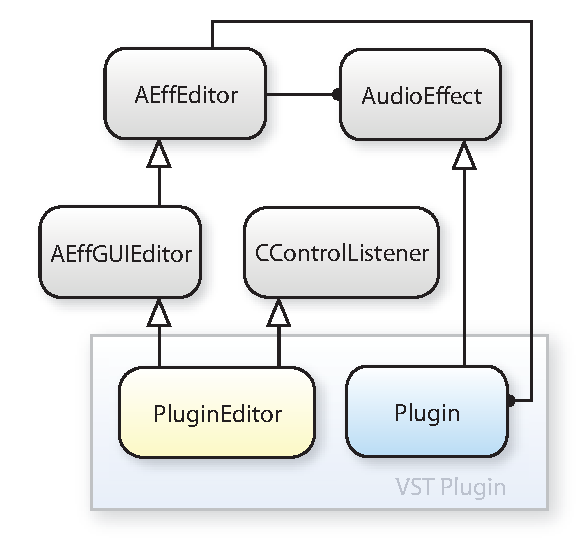
\includegraphics{d02a}}
\caption{\label{obr04} Vzťahy medzi triedami VST SDK}
\end{figure}


\subsection{Knižnica VSTGUI}
VSTGUI je knižnica určená na implementáciu grafického používateľského rozhrania pre pluginy VST a je súčasťou balíka VST~SDK. VSTGUI poskytuje možnosti implementácie platformovo nezávislého používateľského rozhrania. Obsahuje základné ovládacie prvky, napríklad potenciometre, tlačidlá, posúvacie lišty a veľa ďalších. VSTGUI pracuje s grafickými súbormi BMP, vo verzii 3.0 však podporuje aj formát PNG s alfakanálom pre priehľadné a polopriehľadné grafické prvky. K používaniu súborov PNG je nevyhnutné použitie knižníc \emph{libpng}\newfootnote{libpng je knižnica pre podporu formátu PNG. Táto knižnica je závislá na knižnici \emph{zlib}.\newline [http://www.libpng.org]} a \emph{zlib}\newfootnote{zlib je knižnica sprostredkujúca funkcie kompresie a dekompresie dát. [http://zlib.net]}.

Knižnica VSTGUI poskytuje okrem základných komponentov aj abstraktné triedy, ktoré je možné jednoducho použiť na implementáciu vlastných komponentov. VSTGUI ponúka aj základné funkcie pre vykresľovanie primitívnych grafických tvarov a textov. Toto vykresľovanie je ale pod platformou Windows veľmi zastaralé a nepodporuje pokročilejšie funkcie, ako napríklad antialiasing\newfootnote{Antialiasing v kontexte grafiky je odlišný problém, ako pri vzorkovaní zvuku. V grafike ide o spôsob vykresľovania grafických elementov s vyhladzovaním okrajov objektov metódou miešania farieb objektu a pozadia.}. 

\section{Spôsoby tvorby VST syntetizátorov}

Od vzniku rozhrania VST bolo dlhé roky nutné ovládať programovacie jazyky, infraštruktúru operačného systému a mnoho iných vecí na vytvorenie nástroja pre toto rozhranie. V dnešnej dobe ale už existujú aj rôzne vizuálne prostredia, ktoré značnou mierou zjednodušujú tvorbu týchto nástrojov.

\subsection{Vizuálne prostredia pre tvorbu VST}

Najznámejšie vizuálne prostredia sú \emph{SynthEdit}\newfootnote{SynthEdit -- [http://www.synthedit.com]} a oveľa modernejší \emph{SynthMaker}\newfootnote{SynthMaker -- [http://synthmaker.co.uk]} od firmy \emph{Outsim}. Tieto prostredia poskytujú nástroje pre rýchly vývoj syntetizátorov a efektov, veľké množstvo predprogramovaných komponentov a možnosti doprogramovania vlastných komponentov. Tvorba zložitých nástrojov v takýchto prostrediach ale trpí nižšou efektivitou kódu a vyšším zaťažením procesora. Obidve spomenuté prostredia sú komerčné a cena prostredia SynthMaker je rôzna pre osobné a pre komerčné účely.

\subsection{Knižnice a frameworky pre tvorbu VST}

Priamou kompiláciou efektívne navrhnutého kódu je možné dosiahnuť vyšší výkon VST nástrojov, ako pri tvorbe vo vizuálnom prostredí. Tu je ale nevyhnutná pokročilá znalosť programovania, programovacieho jazyka a architektúry operačného systému a hardvérových platforiem, pre ktoré sa nástroj vyvíja.

Pre programovanie a kompiláciu VST nástrojov existujú knižnice a frameworky pre jazyky:

\begin{description}
\setlength{\itemsep}{-0.5ex}
\item[C++] -- VST SDK,
\item[Delphi] -- Delphi VST SDK\newfootnote{Delphi VST SDK -- [http://www.tobybear.de/d\textunderscore template]} je framework pre Delphi, ktorý obsahuje vylepšenia a zjednodušenia originálneho VST SDK pre C++,
\item[Java] -- jVSTwRapper\newfootnote{jVSTwRapper -- [http://jvstwrapper.sourceforge.net]} je wrapper tried VST SDK pre programovací jazyk Java.
\end{description}

Vzhľadom na to, že aj programovacie prostredia sú väčšinou komerčné a ich cena často niekoľkonásobne prevyšuje vizuálne vývojové prostredia, určite je pre záujemcov, ktorí nemajú ambície vyvíjať zložité profesionálne nástroje, výhodnejšie zakúpiť jedno z uvedených vizuálnych prostredí.